% !Mode:: "TeX:UTF-8"
%% 请使用 XeLaTeX 编译本文.
% \documentclass{WHUBachelor}% 选项 forprint: 交付打印时添加, 避免彩色链接字迹打印偏淡. 即使用下一行:
  \documentclass[forprint]{WHUBachelor}

  \begin{document}
  %%%%%%% 下面的内容, 据实填空.
  
  \miji{ 2016级}                                      % 密级. 没有就空着.
  \StudentNumber{16337259(谢江钊)} % 填写自己的学号
  
  \title{基于流水线CPU的分支预测技术性能研究}
  \Etitle{Research on the Performance of Branch Prediction Technology Based on Pipeline CPU} % 英文题目
  \author{谢江钊}                            % 作者名字
  \Eauthor{Xie Jiangzhao}            %作者英文名
  \Csupervisor{李国桢\quad 教授}        %指导教师中文名、职称
  \Esupervisor{Prof.~Li Guozhen}     %指导教师英文名、职称
  \Cmajor{计算机类}                  % 专业中文名
  \Emajor{Computer Class}% 专业英文名
  \Cschoolname{数据科学与计算机学院}          % 学院名
  \Eschoolname{School of Data and Computer Science} %学院英文名. 不确定的话, 请看一下自己学院的网页上是怎么写的. 别搞错了!
  \date{二〇一八年一月}                    % 日期, 要注意和英文日期一致!!
  \Edate{January, 2018}                       % 英文封面日期
  
  %-----------------------------------------------------------------------------
  \pdfbookmark[0]{封面}{title}         % 封面页加到 pdf 书签
  \maketitle
  \frontmatter
  \pagenumbering{Roman}              % 正文之前的页码用大写罗马字母编号.
  %-----------------------------------------------------------------------------
  % !Mode:: "TeX:UTF-8"

%%% 此部分需要自行填写: (1) 中文摘要及关键词 (2) 英文摘要及关键词
%%%%%%%%%%%%%%%%%%%%%%%%%%%%%
%%% -------------  英文封面 (无需改动)-------------   %%%
%%%%%%%%%%%%%%%%%%%%%%%%%%%%%
\thispagestyle{empty}
\renewcommand{\baselinestretch}{1.5}  %下文的行距
\vspace*{0.5cm}
\begin{center}
{\Large \bf Computer Organization Theory \\[1ex] Course Essay }
\end{center}
\vspace{2.5cm}
\begin{center}{\zihao{2} \the\Etitle \par}\end{center}

\vfill

\begin{center}
\zihao{4}
\begin{tabular}{ r l }
 School (Department): & {\sc \the\Eschoolname}\\
  Major:          &   {\sc\the\Emajor}  \\
 Candidate:      &  {\sc \the\Eauthor}      \\
 Supervisor:     &  {\sc \the\Esupervisor}
\end{tabular}

\vspace*{2cm}
\begin{center}
   \ifprint % 文档打印, 使用黑白校徽.
  
\includegraphics[height=4cm]{sysu.pdf}       %%  黑白的.
  \else
  
\includegraphics[height=4cm]{sysu.pdf} %%  彩色的.
  \fi
\end{center}


\zihao{-2}
%\the\Schoolname\\
{\sc Sun Yat-sun University}

\vspace*{1.0cm}

\the\Edate

\end{center}
%%% 郑重声明部分无需改动

%%%---- 郑重声明 (无需改动)------------------------------------%
\newpage
\vspace*{20pt}
\begin{center}{\ziju{0.8}\textbf{\songti\zihao{2} 郑重声明}}\end{center}
\par\vspace*{30pt}
\renewcommand{\baselinestretch}{2}

{\zihao{4}%

本人呈交的论文, 是独立进行研究工作所取得的成果,
所有数据、图片资料真实可靠. 尽我所知, 除文中已经注明引用的内容外,
本论文的研究成果不包含他人享有著作权的内容.
对本论文所涉及的研究工作做出贡献的其他个人和集体,
均已在文中以明确的方式标明. 本论文的知识产权归属于培养单位.\\[2cm]

\hspace*{1cm}本人签名: $\underline{\hspace{3.5cm}}$
\hspace{2cm}日期: $\underline{\hspace{3.5cm}}$\hfill\par}
%------------------------------------------------------------------------------
\baselineskip=23pt  % 正文行距为 23 磅
%------------------------------------------------------------------------------





%%======中文摘要===========================%
\begin{cnabstract}
在文章中我对CPU发展历史以来所采取的预测策略进行了软件上的模拟,对流水线CPU动态预测的性能作出了分析统计。关于此次的CPU设计,我实现了32位MIPS指令集。在学习CPU设计过程中,
流水线CPU的出现极大地提高了CPU的执行效率,但同时也需要合理解决三大冲突。对于控制冲突而言,需要做到尽可能准确预测。近代CPU在
这一方面做分支预测已经非常准确,但是流水线深度的逐渐增加使得哪怕微小的提升也将极大影响CPU的性能。因此文中对过往和近年来热门的预测方法作出评价。\par
为了减少工作量,我采用Python作为工具来解决这个问题。软件层面上我实现了对MIPS汇编程序的模拟执行,并对预测效果作出了统计。\par
分析结果表现混合分支预测器的性能非常优越,相比于传统的局部分支预测和全局分支预测,能够在更短时间内提高预测率并且拥有更加稳定准确的预测正确率。\par
文中的分析结果提供了一种可行性高的办法来评价CPU预测采取策略,可以作为探究分支策略效果的一种手段。


\end{cnabstract}
\par
\vspace*{2em}


%%%%--  关键词 -----------------------------------------%%%%%%%%
%%%%-- 注意: 每个关键词之间用“;”分开,最后一个关键词不打标点符号
\cnkeywords{计算机组成原理; 流水线CPU; 动态分支预测;  }


%%====英文摘要==========================%


\begin{enabstract}
  In the article, I have carried on the software simulation to the forecast tactics that has taken since the CPU development history, has carried on the analysis statistics to the pipeline CPU dynamic forecast performance. About this CPU design, I have realized 32 MIPS instruction set. In learning CPU design process,
  The advent of pipelined CPUs has greatly increased the efficiency of CPU implementation, but at the same time it also requires a reasonable solution to the three major conflicts. For control conflicts, forecasts need to be as accurate as possible. Modern CPU in
  Branch prediction is already very accurate on the one hand, but the gradual increase in pipeline depth makes even a small increase will greatly affect the CPU performance. Therefore, the text in the past and in recent years the popular prediction method to make an assessment. \par
  In order to reduce the workload, I use Python as a tool to solve this problem. At the software level, I implemented the simulation of the MIPS assembler and made statistics on the predicted results. \par
  The results of the analysis show that the performance of the hybrid branch predictor is superior. Compared with the traditional local branch prediction and global branch prediction, the hybrid branch predictor can improve the prediction rate in a shorter time and has a more stable and accurate prediction accuracy. \par
  The analysis results in this paper provide a highly feasible way to evaluate the CPU prediction strategy, which can be used as a means to explore the effect of the branch strategy.

\end{enabstract}
\par
\vspace*{2em}

%%%%%-- Key words --------------------------------------%%%%%%%
%%%%-- 注意: 每个关键词之间用“;”分开,最后一个关键词不打标点符号
 \enkeywords{Computer composition principle; Pipeline CPU; Dynamic branch prediction  }
    % 加入摘要, 申明.
  %==========================把目录加入到书签==============================%%%%%%
  \pdfbookmark[0]{目录}{toc}
  \tableofcontents
  \mainmatter %% 以下是正文
  %%%%%%%%%%%%%%%%%%%%%%%%%%%--------main matter-------%%%%%%%%%%%%%%%%%%%%%%%%%%%%%%%%%%%%
  \chapter{绪论}
  \section{流水线CPU中的控制冲突}
	流水线CPU是多周期CPU的下一步拓展,相比较于多周期CPU,在同一时间内处理多条指令的不同阶段,充分利用了CPU各个部件,
从而加速了程序的执行。但是流水线CPU同样也带来了问题,即我们所讨论的:数据冲突,控制冲突和结构冲突。其中,数据冲突可以通过
设计旁路,流水线暂停技术来解决;结构冲突可以通过分别设置指令存储器和数据存储器来解决。\par
本文章的关键点在于如何解决控制冲突,即由条件分支beq,bne引发的控制冲突。流水线CPU在处理冲突时,需要等到EXE阶段才能够
确定下一条指令的地址。如果我们选择插入冒泡的办法,那么这段时间内的运算能力就会被完全浪费。而如果我们选择预测执行,如果
预测成功就可以保留运算结果,否则就要清空流水线。因此,提升预测的准确率对流水线CPU的性能起到非常关键的作用。\par
	流水线CPU的设计由徐正金解决,但是并没有在Verilog上实现分支预测,这一点恳请老师见谅。
\begin{figure}[ht]
  \centering
    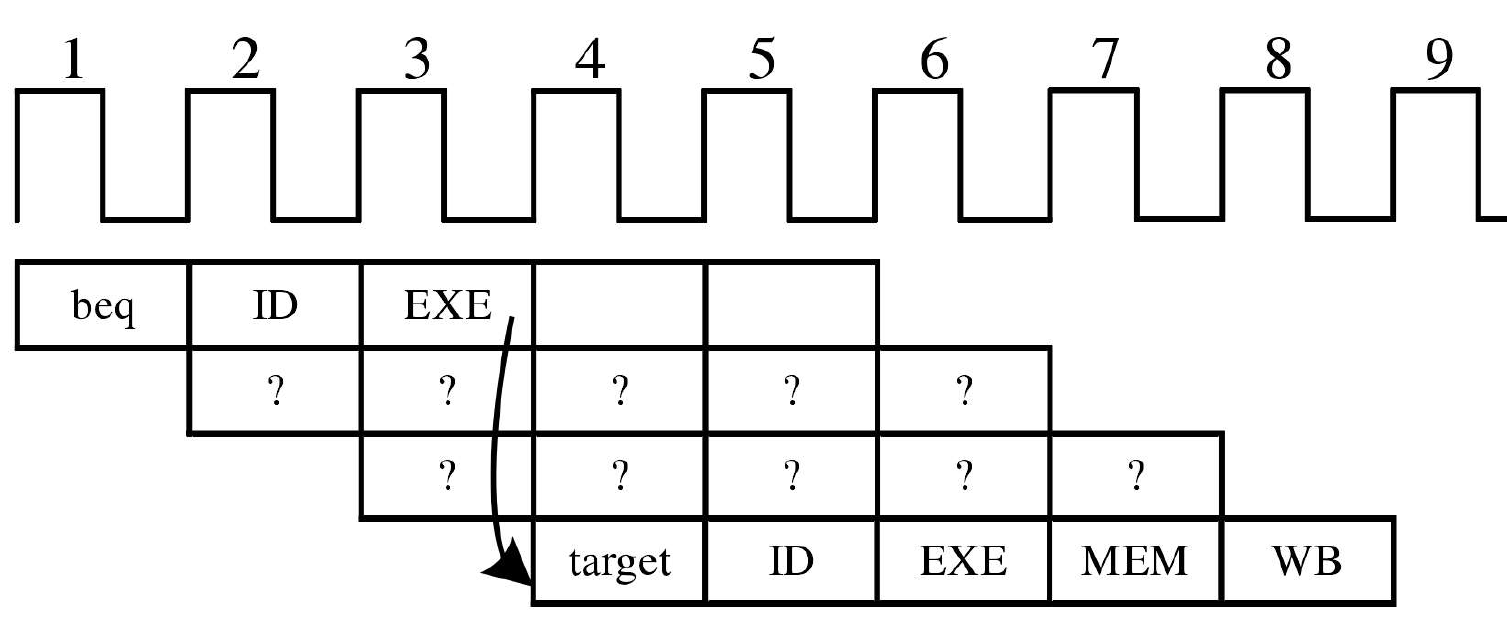
\includegraphics[width=\textwidth]{Conflict.png}
    \caption{控制冲突\upcite{r4}}
    \label{fig:1}
  \end{figure}
   \section{分支预测算法的意义}
  
   分支预测器的重要性在课本中已经得到相当详尽的论述,在这里就不再从原理上去解释它了。回到工业生产中去,
近年来CPU的发展是巨大的,技术的更新集中在更高的制程,频率,深流水线,指令集并行,超线程技术等等上。其中
的流水线加深,更是使得条件分支带来的控制冲突变得日趋严重。分支预测进行得不准确,意味着预测的指令全部都
要抛弃不再进行,这一点会导致极大的性能浪费。其中,奔腾4便是一个失败的例子。奔腾4采用的31级超长流水线,
把主频提高到了3Ghz以上,但是性能却比不过同时期低主频14级流水线的AMD处理器,其中一个重要的原因便是没有
采用高效的分支预测器,导致流水线中断问题极其严重,导致了性能的严重下降。今天的CPU普遍采用14-16级流水线原因之一,
便是分支预测技术瓶颈。\par
业界引入了动态分支预测技术,开发出多种预测方案,使得控制冲突逐渐得到解决。其中较为贴近现代的便是局部分支
预测器,全局分支预测器,循环分支预测器以及间接分支预测器等等,在这里我将对一部分方案作出解释。另外,由
S. McFarling提出的混合(融合)分支预测器相比之下会有更加好的预测结果,同样非常值得考虑作为CPU预测器
发展的方向。\par
更前沿地,当前高端CPU已经迈进了神经网络预测以及多种预测器相结合的道路,在这里由于技术过于复杂便不再进行赘述。
预测器的发展需要考虑到速度和效果,这一点也是需要企业来进行权衡的。如何平衡两者的关系,也是未来发展的一个重点。
做这个项目的时候感触良多,对指令执行特点和CPU自身设计有了很多的体会。而这一个项目实现的内容将来也能够不断改进,
作为未来的教学预测性能预测手段。
  \section{技术发展现状与趋势}\label{sec-compile}

  \subsection{静态分支预测技术}
静态分支技术是最简单的技术,分为两种,强制跳转或强制不跳,而不依赖于过去的历史记录。后来的技术变得更加复杂,假定了
向后分支必然发生,而向前的分支不会发生,对应着程序设计中经常使用到的for循环和if判断特性,能够更好地进行预测。在
早期的时候一些处理器甚至允许分支预测提示出现在代码中,但是后来便不再采用。对于这种做法,理论上是不应该存在的,对于
程序员来说,底层的CPU实现应该做到透明,而不是反过来去负责做分支预测。\par
静态分支预测技术的优点在于对硬件实现基本没有要求,但是预测的效果却见不得理想,尤其对于日渐复杂的程序而言,其准确率
是不能够被接受的。


  \subsection{1bit分支预测器}
1bit分支预测器引入了一位分支预测缓存,记录分支最后一次的选择,然后预测下一次也做出同样的决定。但是这种预测方法有一个
问题在于,如果遇到TFTFTFT...的情况,会造成大量的空翻,从而使得性能被严重浪费。并且由于其总是预测分支跳转/不跳转一定
发生,一旦出现例外情况就会造成两次错误。为了解决这个问题,引入2bit分支预测器,来给预测引入一个缓冲区域。

  
  
  
  \subsection{2bit分支预测器}
2bit分支预测器是基于饱和计数器进行的,饱和计数器是一个拥有4个状态的状态机:强跳转,弱跳转,弱不跳转,他们之间的相互转换关系如下:\par
\begin{figure}[ht]
  \centering
    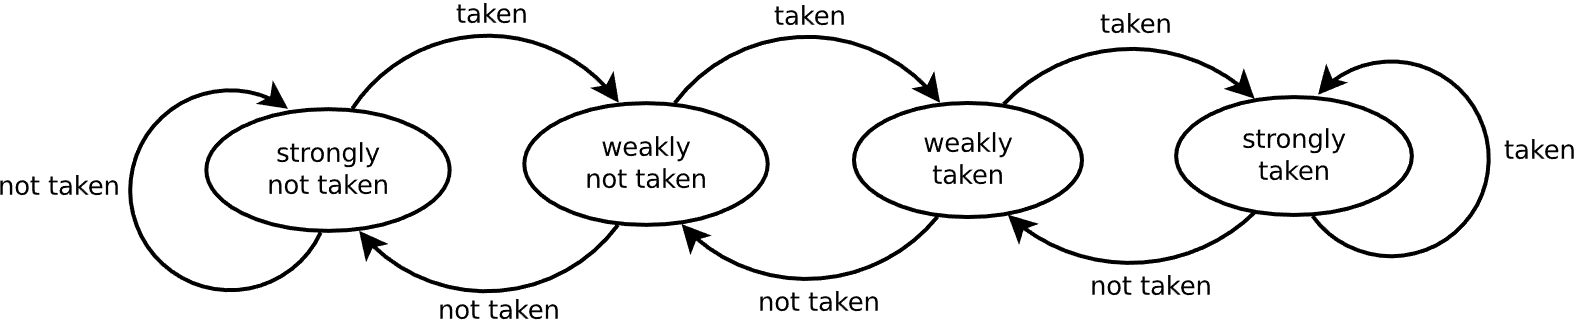
\includegraphics[width=\textwidth]{Counter.png}
    \caption{饱和计数器\upcite{r2}}
    \label{fig:1}
  \end{figure}
2bit分支预测器以跳转指令的PC地址作为索引,然后查找到对应的饱和计数器,根据高位输出结果:\par
\begin{figure}[ht]
  \centering
    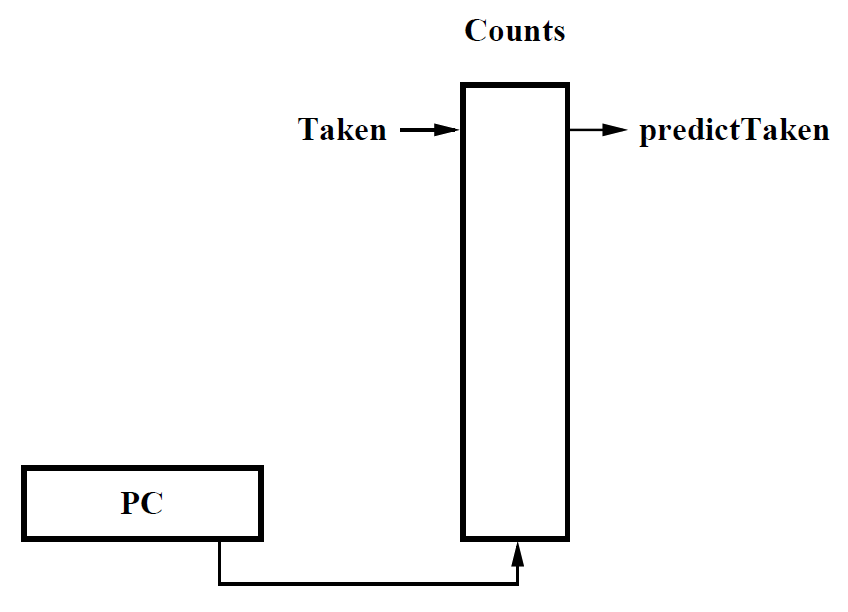
\includegraphics[width=\textwidth]{2bit.png}
    \caption{2bit分支预测器\upcite{r1}}
    \label{fig:2}
  \end{figure}
这种方法的优点在于指令必须选择某个分支连续两次,才能够实现状态的翻转,进而改变预测的分支。回到刚才的情况,一开始的时候
饱和计数器处于强跳转的状态,那么一次F的影响只能使计数器回到弱跳转状态,避免了接连的空翻,相比之下错误率下降。同样的道理,
我们还可以提出nbit分支预测器,来给予更多的缓冲空间,但是这种做法也导致了跳转不能够灵活地得到改变,在测试中反而导致预测率
下降。

 \subsection{局部分支预测器}
 前面所描述的2bit分支预测器,用状态机的办法把过去若干条指令改变的结果保存了下来,但是这样有一个问题,认为本次的跳转与
 之前的若干条指令跳转有关,但是处理起来却把本次预测结果应该基于过去的情况。举个例子,假如之前的几次跳转结果是TTF,那么
 这一次的结果如果仅仅看作前几次的衍生的话,便有可能出错。例如对于一个循环而言,循环3次跳转最后一次不跳转(跳出循环),如果
 依靠2bit分支预测器就会出现预测错误的结果,因为前三次的跳转不能够表明这一次也一定跳转。相对应的是,我们可以把前三次的历史
 记录看作是一种模式,然后在此基础上构建饱和计数器,经过若干次训练,便可以得到一个结果:三次的跳转必然伴随着一次结果,这样我们
 往后的预测便会变得准确,提高了我们的正确率。\par
 \begin{figure}[ht]
  \centering
    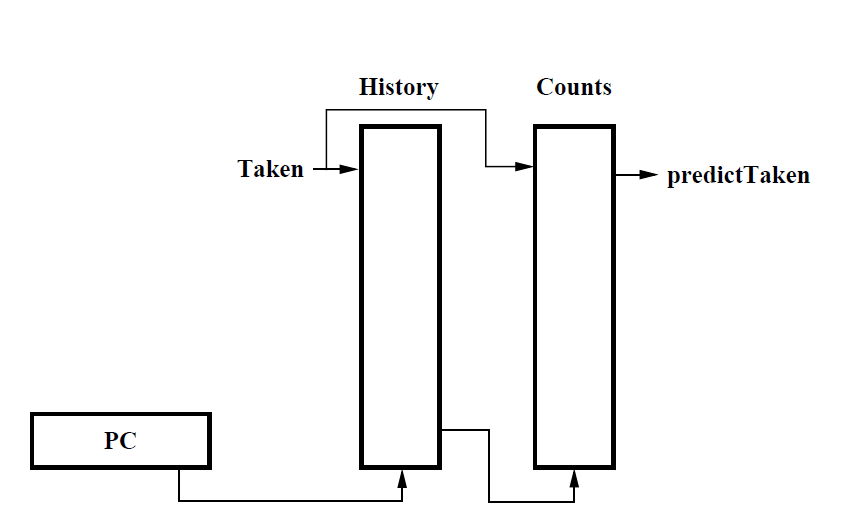
\includegraphics[width=\textwidth]{Local.png}
    \caption{局部分支预测器\upcite{r1}}
    \label{fig:3}
  \end{figure}
 局部分支预测器构建了两个表:一个被称为BHT(Branch History Table),另一个被称为BPT(Branch Pattern Table)。BHT以跳转指令的
 地址作为索引,记录改分支的历史记录,然后根据分支的历史记录去查询对应的饱和计数器,根据计数器的高位进行相对应预测。预测的结果
 同样会不断更新历史和计数器。在经过大量训练后便可以得到相当优秀的正确率。这种预测方式被现代CPU普遍地采纳。

 \subsection{全局分支预测器}
 局部分支预测器仅仅通过指令自身的预测历史预测了指令的跳转,但是却没有考虑到指令之间的相关性。对于某些指令,例如\par
 if(a>0) todo;\par
if(a<=0) todo;\par
第一条指令和第二条指令必然只会发生一条,通过观察第一条指令的跳转情况便可以预测第二条指令的跳转结果。对于一个不断变化的a,这个
时候局部分支预测器便不能仅仅通过自身的历史记录来推测出下一次跳转情况。因此,全局分支预测器采取的做法是,记录下前几条指令的跳转情况,
然后通过这个历史记录来查找对应的饱和计数器,从而解决了跳转指令的相关问题。\par
全局分支预测器通过GR(Global History)来索引饱和计数器,获得对应的预测结果。\par
\begin{figure}[ht]
  \centering
    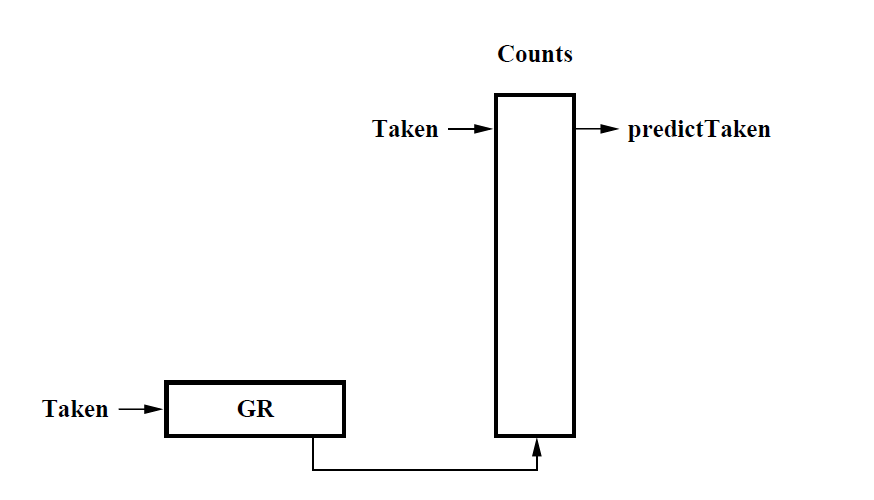
\includegraphics[width=\textwidth]{Global.png}
    \caption{全局分支预测器\upcite{r1}}
    \label{fig:3}
  \end{figure}

\subsection{混合分支预测器}
相比以上两种分支预测器,混合分支预测器仅仅是简单地将他们组合起来,从而在面对复杂的分支情况时能够更有效地采取不同的预测器,获得更加优秀
的表现。混合分支预测器将预测的任务分别交给全局分支预测器和局部分支预测器去预测,然后根据它们的预测结果以及预测的指令地址,来更新自己的
索引表,这个表记录着若干的饱和计数器\upcite{r1},饱和计数器的状态决定了全局分支预测器决定要采纳哪一种预测结果。
\begin{figure}[ht]
  \centering
    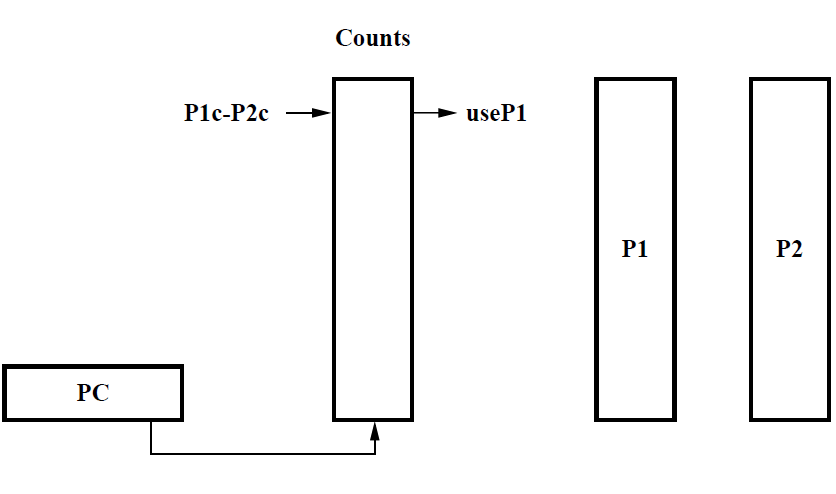
\includegraphics[width=\textwidth]{Merge.png}
    \caption{混合分支预测器\upcite{r1}}
    \label{fig:3}
  \end{figure}

\subsection{基于上述分支预测器的优化}
由于硬件方面的限制,上述分支预测器的索引不可能直接取到整个PC的大小,相对地,我们会采用记录PC低位的方法来作为表的索引。对于全局历史分支
预测器,还发展出了PC地址和GR记录做异或的方法来作为索引,这种做法能更好地避免冲突。但是受制于所写汇编程序的大小,相关的优化也就没有进行。
对于PC地址我做了对32取模,用来作为索引。

  
  \chapter{分支预测算法的软件实现与验证}
  
  \section{32位MIPS指令集实现}
  指令集方面我实现了所有32位MIPS指令:
      
    \begin{itemize}
      \item R型指令:add,addu,sub,subu,and,or,xor,nor,slt,sltu,sll,srl,sra,sllv,srlv,srav,jr
      \item I型指令:addi,addiu,andi,ori,xori,lui,lw,sw,beq,bne,slti,sltiu
      \item J型指令:j,jal
    \end{itemize}
    \par
    至于更具体的细节可以参考\url{http://blog.csdn.net/yixilee/article/details/4316617}
    在实现文件中,对读入的每条指令分解为opcode,rs,rt,rd,reserved等部分,
    从而实现对指令的译码,这一点与硬件上保持一致。关于软件的更多细节在此不再赘述,项目的详细文档可以在
    \url{https://github.com/xiejiangzhao/MIPS_Predict}获取,在此基础上还可以加入对x86指令集,新增其他预测方法的支持。\newpage
  
\section{不同预测方法的效果测试}
  以下对包括多重循环,排序算法等汇编代码进行了测试。\\
  \begin{figure}[ht]
    \centering
      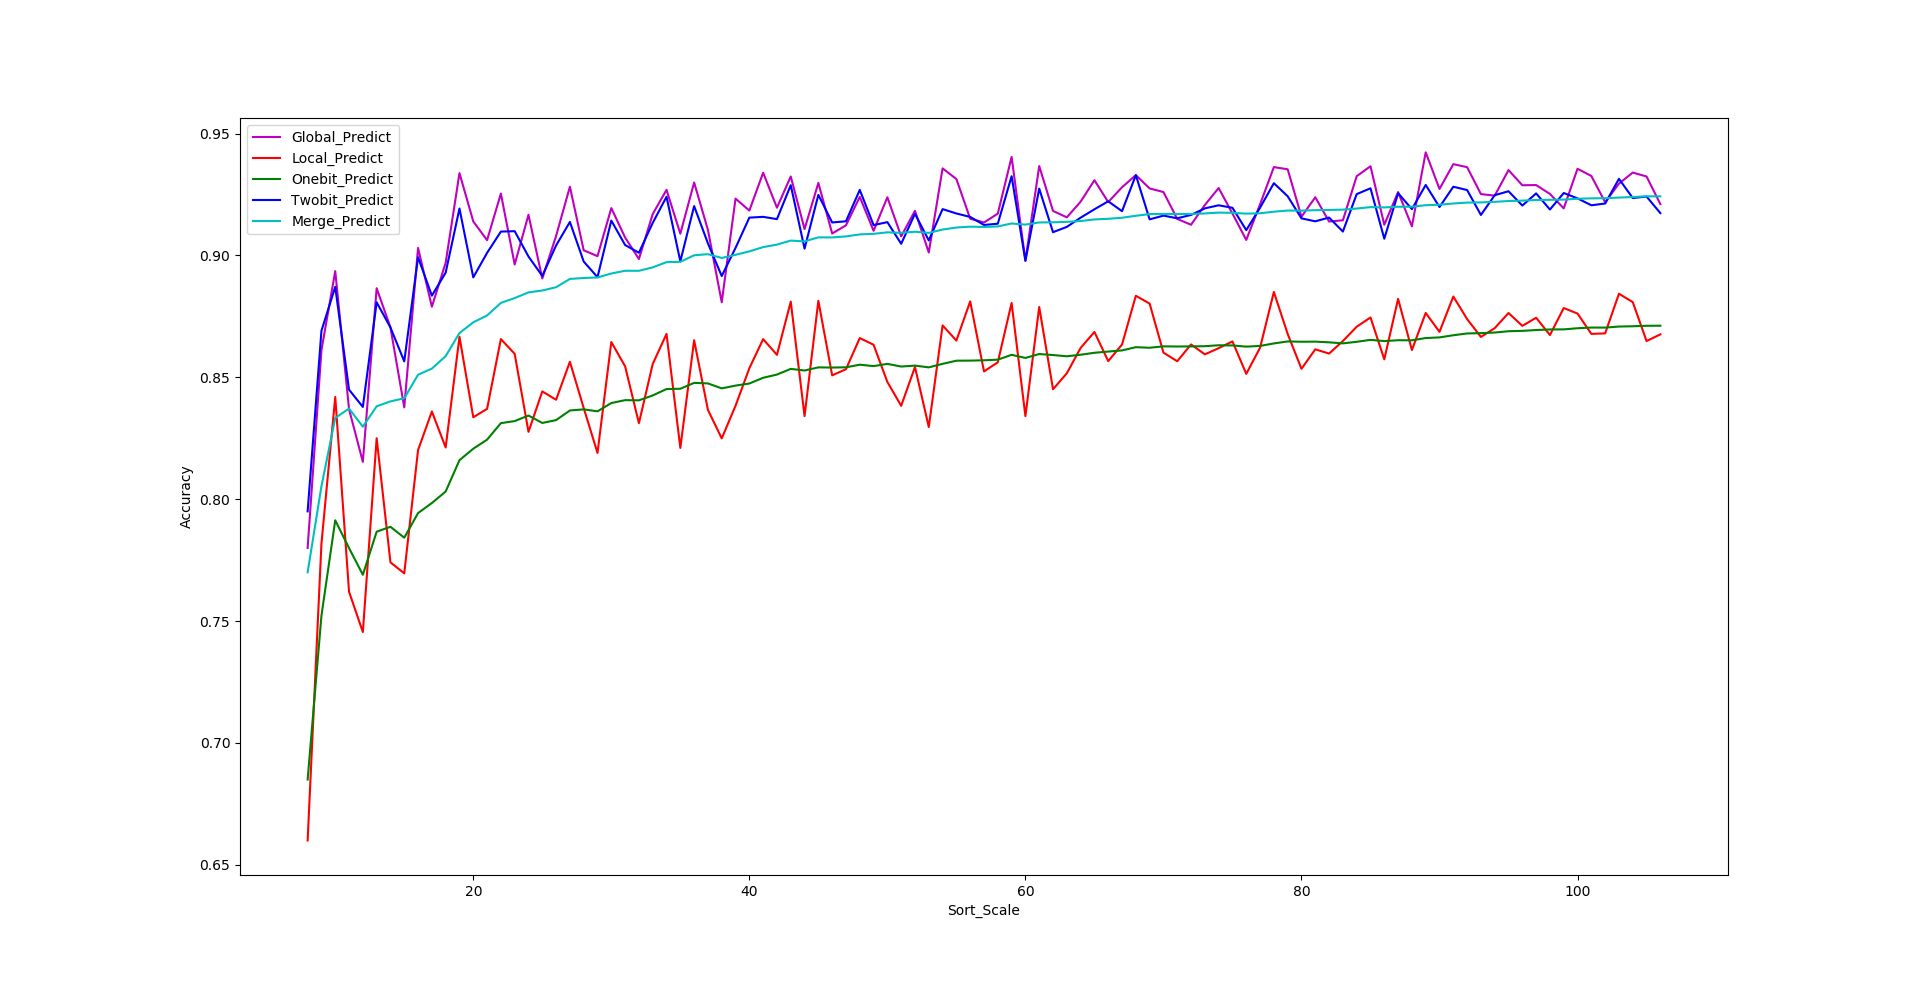
\includegraphics[width=14cm]{Figure_1.png}
      \caption{冒泡排序预测结果}
      \label{fig:1}
    \end{figure}
  \begin{figure}[ht]
    \centering
      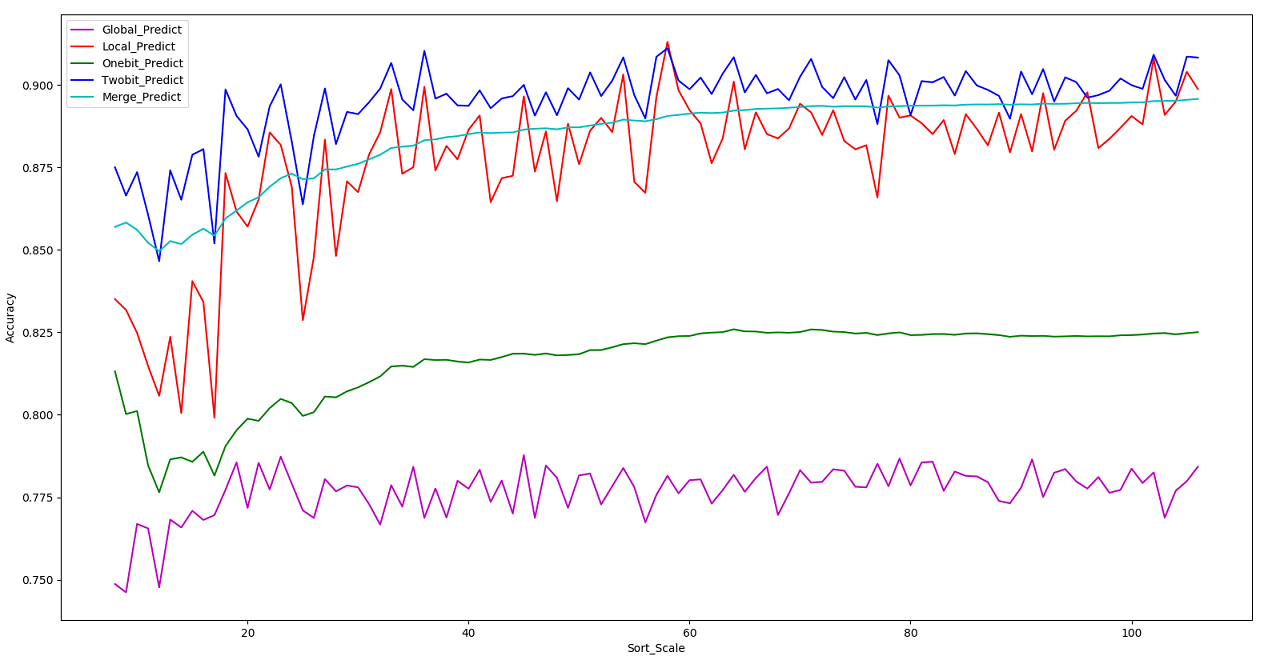
\includegraphics[width=14cm]{Figure_2.png}
      \caption{多层循环+TF变化预测结果}
      \label{fig:1}
    \end{figure}
  \begin{figure}[ht]
    \centering
      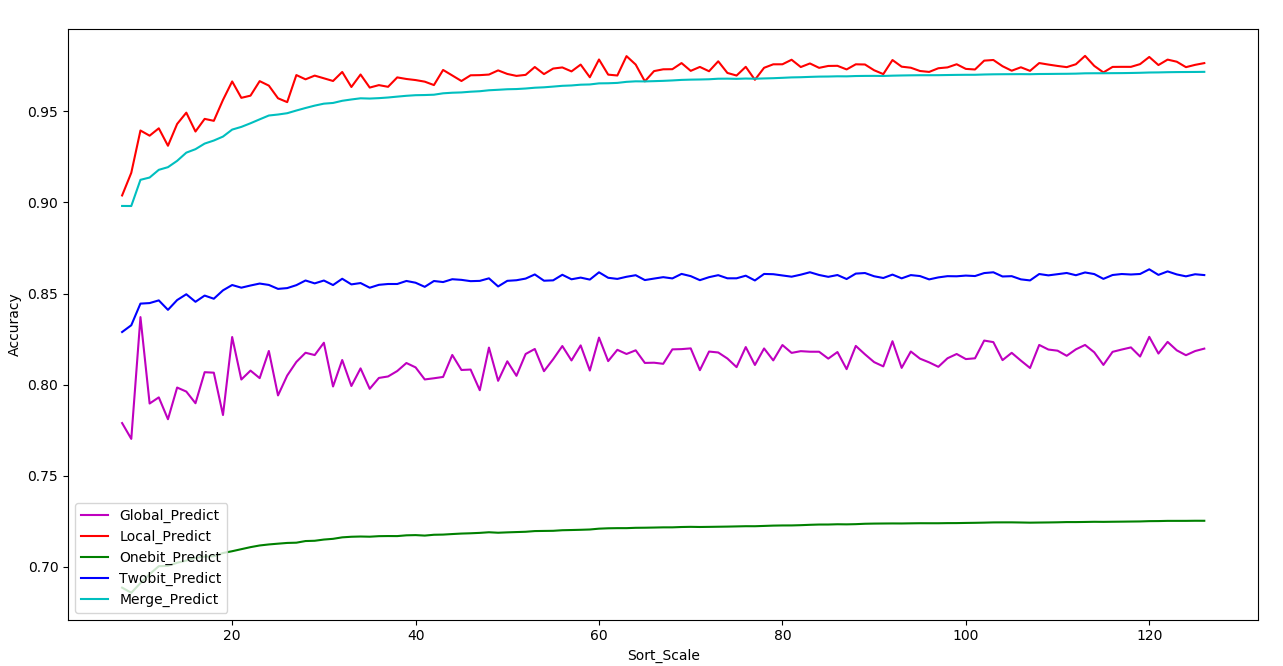
\includegraphics[width=\textwidth]{Figure_3.png}
      \caption{规律跳转预测结果}
      \label{fig:1}
    \end{figure}
  \section{预测结果评价}
  由预测结果,可见在不同的场景下预测器取得的效果是不同的,甚至差异性比较大。
  图表中值得留意的一点是,尽管混合分支预测器不能极大地提高正确率,但是预测效果较为稳定,在不同的场景下都能够取得
  相对优秀的结果。在实际生产环境中,跳转情景将会比上述情况更为复杂,这种不确定性都将会使得单一的分支预测效果
  不同程度下降,而混合分支预测器则能够较好地去拟合它们。

  %%%%============================================================================================================%%%
  
  \chapter{项目总结}
  透过这个项目,了解到了很多课本及其以外的动态分支预测的手段,通过建表,引入更加复杂的索引方式来在有限的硬件资源中取得更好的效果。分支预测相比一开始已经走了很远的路,同时各类消除冲突的手段诸如乱序执行等等也进一步避免了冲突的产生,但分支预测的发展却从未终止。这一点还是像一开头所说的,得益于流水线发展以及程序的复杂性不断提高。尤其对于某些体积相当大的软件来说,过小的分之历史表会导致像缓存失效一样的结果:相互之间干扰会变多。\par
关于分支预测的发展我作了几点思考,它的未来要如何去发展:1.首先是算法的改进,利用目前更加高效的诸如神经网络算法等等手段去提高它的准确率。2.是否可以考虑缓存机制来提升分支预测的效果,对MIPS而言,它的跳转取决于寄存器的值的比较,而这些是可以异步去做的。3. 编译器层面上是否可以进一步去改进,从编译器的层面上去尽可能减少冲突或者令跳转更加可预测。以上,我认为将能够使得未来发展更深流水线CPU时能够避免分支预测错误带来的性能浪费。\par
这个项目本身存在不足之处,受制于时间和电脑性能的约束,没有能力对各类平台和各种大小的预测器做大规模的汇编程序测试,关于这一点深感遗憾,在这里致以歉意。\par
分工方面谢江钊实现了软件层面上利用Python对分支预测器性能的测试和数据统计,包括论文的编写;徐正金在Verilog上实现了无分支预测流水线CPU。
  
  %%%============================================================================================================%%%
  
  %%%=== 参考文献 ========%%%
  \cleardoublepage\phantomsection
  \addcontentsline{toc}{chapter}{参考文献}
  \begin{thebibliography}{00}
  
    \bibitem{r1} Scott McFarling,Combining Branch Predictors,WRL Technical Note TN-36, 1993.
  
    \bibitem{r2} Wikipedia,\url{https://en.wikipedia.org/wiki/Branch_predictor}.
  
    \bibitem{r3} 沙子岩,基于神经网络的处理器分支预测技术研究,2010
  
    \bibitem{r4} 秘海晓,基于FPGA的32位五级流水线CPU的研究与设计,2012
  
  
  
  \end{thebibliography}
  
  % !Mode:: "TeX:UTF-8"
%%%%%%%%%%%%%%%%%%%%%%%%%%%%-------致谢--------%%%%%%%%%%%%%%%%%%%%%%%%%%%%%%%%

\acknowledgement
\addcontentsline{toc}{chapter}{致谢}


感谢你, 感谢他和她, 感谢大家.











 %%%致谢
  
  %%%-------------- 附录. 不需要可以删除.-----------
  \appendix
	\chapter{项目相关实现细节}
	\section{分支预测器评价的Python架构}
		
  \end{document}
  
  
  
   